\documentclass[twocolumn]{ltjarticle}
\usepackage[bibstyle=ieee,citestyle=numeric,maxnames=99,maxnames=2,url=true,doi=true,hyperref=true]{biblatex}
\usepackage[dvipdfmx]{graphicx}
\usepackage{amssymb}
\usepackage{eshouroku}
\usepackage{color}
\usepackage{graphics}
\usepackage{amsmath}
\usepackage{subfigure}
\usepackage{url}
\usepackage{upgreek}
\usepackage{bm}
\usepackage{here}
\usepackage{nicematrix}
\usepackage{enumitem}

\boldmaintrue% 主文を太字にするモード(指導教員添削時はこちら)
% \boldmainfalse% 主文を普通文字にするモード(抄録印刷時はこちら)

\addbibresource{ref.bib}

\begin{document}
\twocolumn[
\講演番号{B-XX}% 必要ない場合には書かない
\日本語タイトル{\fontsize{16.1pt}{16.1pt}\selectfont}{ベイズ最適化を用いた通信速度改善のための送信位置設計法}
\英語タイトル{\large}{Transmission Position Design Method for Data Rate Improvement Using Bayesian Optimization}
\筆者一名{5322}{竹中公材}
%\筆者二名{53XX}{産技太郎}{53YY}{品川次郎}
%\筆者三名{53XX}{産技太郎}{53YY}{品川次郎}{53ZZ}{東大井三郎}
%\筆者四名{53XX}{産技太郎}{53YY}{品川次郎}{53ZZ}{東大井三郎}{53WW}{荒川四郎}
\指導教員一名{稲毛契}
%\指導教員二名{東京花子}{京都紀夫}
%\指導教員なし
]

% \addcontentsline{toc}{section}{\refname}% 追加

%\graphicspath{{./figures/}} % 図が特定のフォルダにある場合には設定

\section{はじめに}
私たちが日常的に使用しているスマートフォンやノートパソコンなどの通信機器は持ち運ぶことができ,位置の調整が容易である.
そのため,通信速度が低い場合はその位置を調整することで,通信速度を改善することができる.
しかし,IoT(Internet of Things)の普及に伴い,産業機器や家電製品などに無線通信機能が搭載されることが増えている\cite{soumu}.
これらは複数の箇所に固定設置されていることが多く,位置の調整が困難であるため位置変更により通信速度を向上させるのは容易ではない.
このような固定設置された受信機の通信速度を向上させるには,送信機の数を増やす,あるいは高出力の送信機に替えるといった方法が考えられるが,いずれもコスト(送信機の費用)がかかる.

そこで,送信機の位置を調整して受信機の通信速度を向上させる方法が挙げられる.
電波は距離の累乗に比例して減衰するため,送信機と各受信機間の距離から最適な送信機位置を決定できると考えられる.
しかし,壁や扉などの周囲の構造物による反射や回折により,シャドウイングと呼ばれる短区間の変動が生じ,電波の伝搬が複雑になるため通信速度が距離のみの関数にならず,最適な送信機位置の予測が困難になる.
この短区間の変動をシャドウイングと呼ぶ.

このような場合、送信機位置の予測を行うことは不可能であるため、実際に各受信機の通信速度を測定を行い送信機の位置を決定する必要がある.
具体的な手法としては,送信機位置を全パターンを試すグリッドサーチと呼ばれる手法がある.
この手法は,確実に最適な位置を見つけることができるが,多くの試行回数を必要とするため,非常に多くの時間や労力がかかる.

試行回数をできるだけ少なくするためには,送信機の位置を入力,通信速度(各受信機の中で最も低い値)を出力とする関数と考え,この関数の最大値を求めることが有効である.
屋内の複雑な電波伝搬特性はブラックボックス関数(具体的な形状が不明な関数)であるため,勾配法やニュートン法などの傾きを用いた最適化を適用することが難しい.

そこで本研究では,ブラックボックス関数で最適値を求めることができるベイズ最適化と呼ばれる手法を無線環境測定プロセスに適用し,通信速度と測定回数を改善することを目的とする.
% \section{従来の最適化手法の問題点}

% 最適化とは,ある関数の最大値や最小値を求めることであり,勾配法やニュートン法などを用いる方法がある.
% これらの最適化手法はある関数が\(y=f(x)\)のように数理的な構造が明確であり,傾きを用いるため微分可能であることを前提とする.
% しかし,ブラックボックス関数の場合は明確な関数がわからず微分可能か把握できないため,これらの最適化手法を適用できない.
\section{ベイズ最適化}

ベイズ最適化は,毎回の測定において適切な入力値を確率的に選択し,少ない試行回数で最適値を効率的に探索する手法であり,一回あたりの実験コスト(実験費用や時間)が高い場合に有効な手段である.
適切な入力値を確率的に選択するために,ガウス過程回帰を用いる.
回帰とは,過去の測定点を用いて入力値から出力値を予測することである.

\subsection{ガウス過程回帰}

ガウス過程回帰がブラックボックス関数の最適化に有効である理由として、従来の回帰で必要だった\(y=ax+b\)のようなモデル式を使わずに関数を推定することができることがあげられる.
ガウス過程回帰を用いることで\wfig{gaussian_process}のように赤点の測定点から関数を正規分布に従う確率分布として推定できる.
ここで,青線は推定結果(平均\(\mu\)),薄い青のエリアは68\%の確率で値が存在する区間(標準偏差\(\sigma\))を表す.
ガウス過程回帰は,カーネル関数を用いて関数の形状を推定する.
そのため,ベイズ最適化ではカーネル関数の選択が重要である\cite{gaussian_process}.
\setlength\intextsep{3pt}
\setlength\textfloatsep{3pt}
\begin{figure}[htbp]
	\centering
	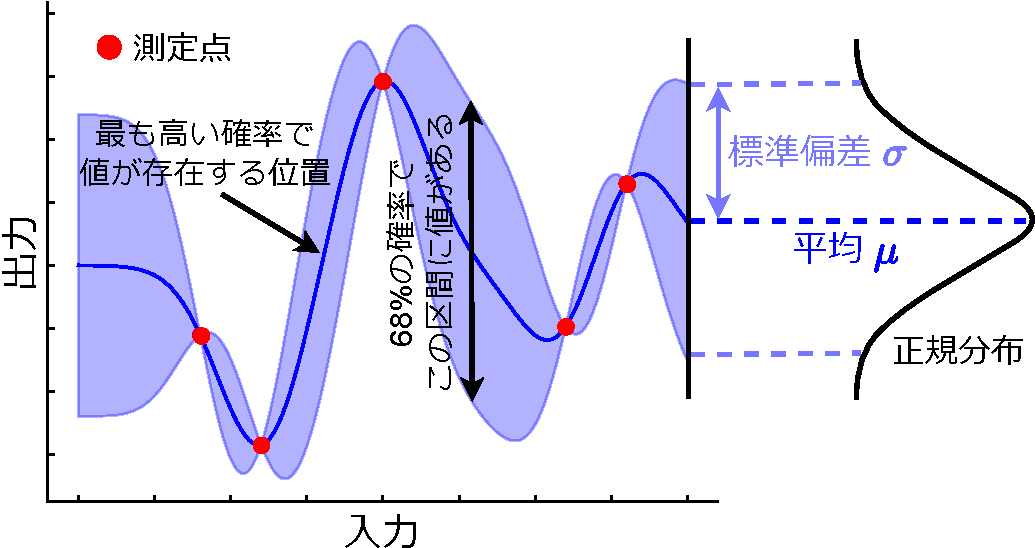
\includegraphics[width=0.83\linewidth]{./figures/material_5_kernel_v2.pdf}
	\vspace*{-0.3cm}
	\caption{ガウスカーネルを用いたガウス過程回帰のイメージ} \label{fig:gaussian_process}
\end{figure}
\subsection{カーネル関数}

カーネル関数は測定点と測定点の間を関連づけるときに用いる類似度を計算する.
本研究では,\weq{matern}のMaternカーネルを用いる.
ここで,\(\nu\)は関数の滑らかさを示すパラメータであり,値が大きいほど滑らかである.
\(\nu=\infty\)でガウスカーネル,\(\nu=1/2\)で指数カーネル,\(\nu=3/2\)でMatern3/2カーネル,\(\nu=5/2\)でMatern5/2カーネルと呼ばれる.
また,\(\Gamma\)はガンマ関数,\(B_{\nu}\)は第二種変形ベッセル関数,\(\theta\)はハイパーパラメータである.
\begin{align}
	\scalebox{1.0}{
		\(
		k(x, x^{\prime}) = \frac{2^{1-\nu}}{\Gamma (\nu)}\left(\frac{\sqrt{2\nu}\Vert x - x^{\prime} \Vert}{\theta}\right)^{\nu} B_{\nu} \left(\frac{\sqrt{2 \nu} \Vert x - x^{\prime} \Vert}{\theta}\right) \label{eq:matern}
		\)
	}
\end{align}
\(\nu\)のパラメータを変更することにより,\wfig{matern_graph}のように入力値間の差\(||x-x^{\prime}||\)と類似度の波形が変化する.
これにより、\wfig{gaussian_process}のようなガウスカーネルを用いた波形と\wfig{exp_kernel}ような指数カーネルを用いた波形を比べると,ガウスカーネルは滑らかな波形になるのに対し指数カーネルは局所的な波形になっていることがわかる.
指数カーネルは他のカーネルに比べて類似度が急激に減少していることが要因となる(\wfig{matern_graph}
\setlength\intextsep{6pt}
\setlength\textfloatsep{6pt}
\begin{figure}[H]
	\begin{minipage}[t]{0.5\columnwidth}
		\centering
		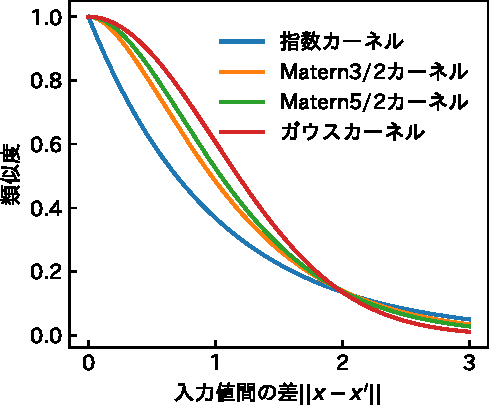
\includegraphics[width=\columnwidth]{./figures/kernel-crop.pdf}
		\vspace*{-0.8cm}
		\caption{各カーネル関数} \label{fig:matern_graph}
	\end{minipage}
	\begin{minipage}[t]{0.47\columnwidth}
		\centering
		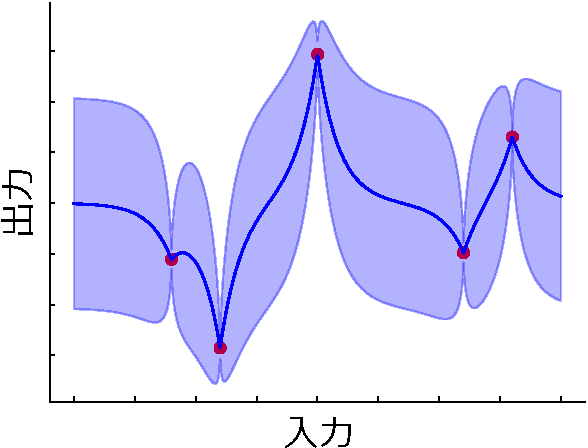
\includegraphics[width=\columnwidth]{figures/material_8_exp.pdf}
		\vspace*{-0.8cm}
		\caption{指数カーネル} \label{fig:exp_kernel}
	\end{minipage}
\end{figure}
\noindent
参照).
このようにカーネル関数を変更することにより,推定した関数の形状が変化するため,対象とするブラックボックス関数に合わせて適切なカーネル関数を選択する必要がある.
\subsection{ベイズ最適化の流れ}

ベイズ最適化では,最初にいくつかの地点を測定する必要がある.
これは,ガウス過程回帰を用いるために入力と出力のデータが必要であるためである.
次に測定したデータを用いてガウス過程回帰を用い,獲得関数を求める.
獲得関数は,次の測定値を決定する関数であり,\weq{acquisition}のように定義される.
ここで,\(\mu\)と\(\sigma\)はそれぞれガウス分布の平均と標準偏差,\(\beta\)は\(\mu\),\(\sigma\)を調整するパラメータであり,任意に設定する係数である.
% 多くの場合,測定回数\(N\)を用いて\(\beta\)は\(\sqrt{\frac{\log N}{N}}\)と定義されることが多いため,本研究でこれを採用する.
\begin{align}
	a(\mu, \sigma, \beta) = \mu + \beta \sigma \label{eq:acquisition}
\end{align}
\weq{acquisition}で定義した獲得関数の最も高い点を次の測定箇所として選択し,選択された測定箇所が既に測定されている場合,その地点を最適値とする.
\section{シミュレーション}

ベイズ最適化が送信機の位置決定において有用であるかを確認するために,シミュレーションを行った.
\subsection{電波伝搬モデル}

フリスの公式と対数正規シャドウイングを用いて電波伝搬環境を作成し,送信機を動かしながらランダムな場所に配置した複数の受信機の通信速度を計算した.
電波が距離の累乗に比例して減衰する特徴を\weq{friss}のフリスの公式で表現する.
ここで,\(\lambda\,\mathrm{[m]}\)は使用する電波の波長,\(\mathrm{d_0}\,\mathrm{[m]}\)は自由空間距離(遮蔽物に当たらない距離),\(\mathrm{d}\,\mathrm{[m]}\)は送受信機間距離,\(n\)は障害物により電波が減衰する程度を示す伝搬係数である.
\begin{align}
	\scalebox{0.9}{
		\(
		\mathrm{P_{LOSS}} =
		\begin{cases}
			20 \log_{10} \left( \frac{\lambda}{4 \pi \mathrm{d}} \right)                                                         & (\mathrm{d < d_0})     \\
			20 \log_{10} \left( \frac{\lambda}{4 \pi \mathrm{d_0}} \right) - 10n \log_{10} \left( \mathrm{\frac{d}{d_0}} \right) & (\mathrm{d \geqq d_0})
		\end{cases} \label{eq:friss}
		\)
	}
\end{align}

シャドウイングは,空間相関性(距離が近いほど似た値を持つ性質)を表す\weq{shadowing}の相関係数\(\rho\)を用いて相関行列を作成し,
その相関行列をコレスキー分解して得られる下三角行列と正規分布に従う乱数との行列積で表現する\cite{shadowing}.
ここで,\(\mathrm{\Delta d_{TX}}\,\mathrm{[m]}\)は送信機の位置の変化量,\(\mathrm{\Delta d_{RX}}\,\mathrm{[m]}\)は受信機の位置の変化量,\(\mathrm{d_{cor}}\,\mathrm{[m]}\)は位置の変化量によって相関を与える程度を示す相関距離である.
\begin{align}
	\rho \approx \exp \left( - \mathrm{\frac{\Delta d_{TX} + \Delta d_{RX}}{d_{cor}}} \ln 2 \right) \label{eq:shadowing}
\end{align}

\weq{friss}と\weq{shadowing}は受信信号強度(RSSI)を計算する式であるため,\weq{capacity}を用いて受信信号強度から通信速度に変換する必要がある.
ここで,\(\mathrm{RSSI}\,[\mathrm{dBm}]\)は受信信号強度,\(\mathrm{Noise}\,[\mathrm{dBm}]\)はノイズフロア,\(B\,[\mathrm{Hz}]\)は帯域幅,\(C\,[\mathrm{bps}]\)は通信速度である.
\begin{align}
	C = B \log_2 \left( 1 + 10^{\frac{\mathrm{RSSI}}{10}-\frac{\mathrm{Noise}}{10}} \right) \label{eq:capacity}
\end{align}
\subsection{シミュレーション環境}

20\(\,\)m\(\times\)20\(\,\)mの空間を用意し,1台の送信機を0.5\(\,\mathrm{m}\)刻みでグリッド状のどこかに設置できるようにした.
また受信機は,空間内のランダムな場所に5つ配置した.
\weq{friss},\weq{shadowing},\weq{capacity}を用いて,入力を送信機の位置,出力を各受信機の中で一番遅い通信速度とした関数を作成した.
その後,ベイズ最適化を行い、グリッドサーチで求めたものを真値として比較した.
ベイズ最適化を用いたときの測定回数,真値との間の距離を調べた.
\section{結果}

\wfig{result_count}にベイズ最適化を用いたときの測定回数の結果、\wfig{result_error}にベイズ最適化を用いたときの真値との差の結果を箱ひげ図として表す,
箱ひげ図では中央値、データの真ん中の50\%区間、最大値、最小値、外れ値が分かる.
結果より、カーネル関数の種類によらずグリッドサーチ(1681回)と比較してベイズ最適化の方が測定回数を少なくすることに成功している.
Maternカーネルの\(\nu\)の値が大きいほど測定回数のばらつきが大きく,平均値も高く、真値からの距離が小さい事が分かる.
このような結果になった要因として、目的関数が指数カーネルのような局所的な波形ではなかったため、上手くフィッティングできなかったためであると考えられる.

\setlength\intextsep{3pt}
\setlength\textfloatsep{3pt}
\begin{figure}[H]
	\centering
	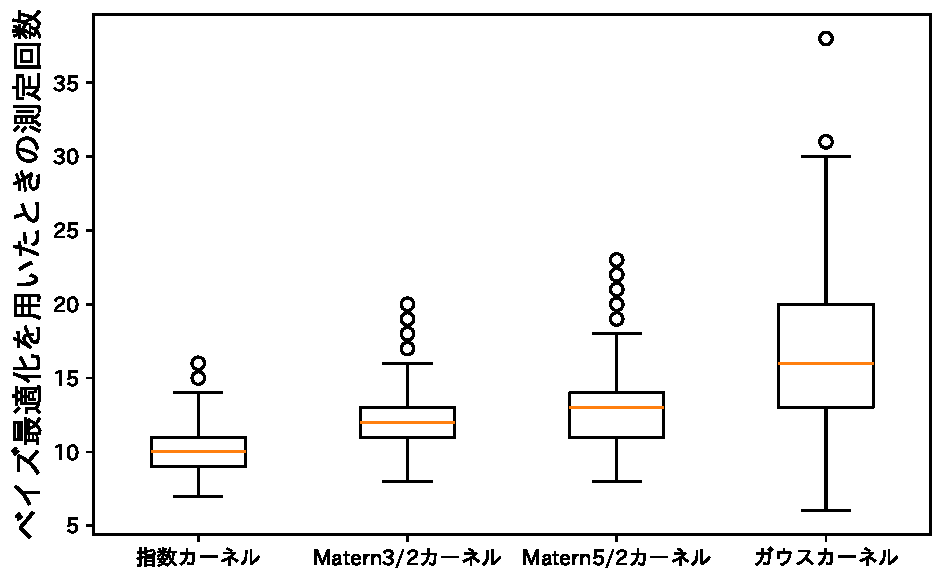
\includegraphics[width=0.83\linewidth]{./figures/count_box.pdf}
	\vspace*{-0.4cm}
	\caption{ベイズ最適化を用いたときの測定回数の結果} \label{fig:result_count}
\end{figure}
\vspace*{-0.1cm}
\begin{figure}[H]
	\centering
	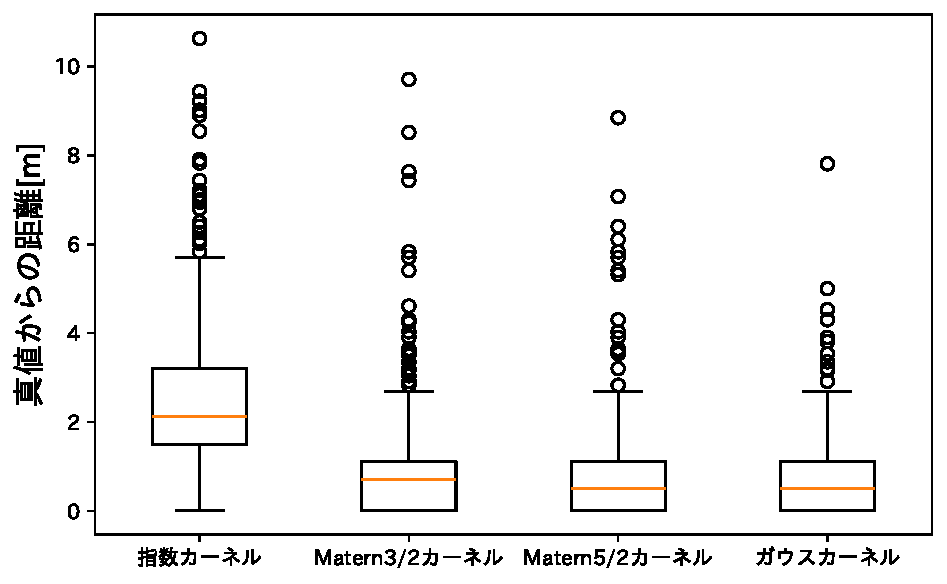
\includegraphics[width=0.83\linewidth]{./figures/dis_box.pdf}
	\vspace*{-0.4cm}
	\caption{真値からの距離の結果} \label{fig:result_error}
\end{figure}

\section{おわりに}

ベイズ最適化を用いて最適な送信機の位置を求める手法を提案し,シミュレーションでその有用性を確認した.
その結果,提案手法は全探索と比較して測定回数を大幅に削減することができた.
4種類のカーネル関数を比較した結果,測定回数と精度はトレード・オフの関係にあり,Matern5/2カーネルがバランスを保てていることがわかった.
\printbibliography[title=参考文献]

\end{document}
